\documentclass[conference,final]{IEEEtran}

\usepackage{latex8}
\usepackage{times}

\usepackage[utf8]{inputenc}
\usepackage{url}
\usepackage{float}
\usepackage{times}    
\usepackage{multirow}    
\usepackage{listings}   
\usepackage{times}     
\usepackage{paralist}    
\usepackage{wrapfig}    
\usepackage[small,it]{caption}
\usepackage{multirow}
\usepackage{ifpdf}
%\usepackage{srcltx}
\usepackage{subfigure}


\usepackage{listings}
\usepackage{keyval}  
\usepackage{color}
\definecolor{listinggray}{gray}{0.95}
\definecolor{darkgray}{gray}{0.7}
\definecolor{commentgreen}{rgb}{0, 0.4, 0}
\definecolor{darkblue}{rgb}{0, 0, 0.4}
\definecolor{middleblue}{rgb}{0, 0, 0.7}
\definecolor{darkred}{rgb}{0.4, 0, 0}
\definecolor{brown}{rgb}{0.5, 0.5, 0}

\newif\ifdraft
\drafttrue
\ifdraft
\newcommand{\jhanote}[1]{ {\textcolor{red} { ***shantenu: #1 }}}
\newcommand{\alnote}[1]{ {\textcolor{blue} { ***andre: #1 }}}
\newcommand{\smnote}[1]{ {\textcolor{green} { ***sharath: #1 }}}
\newcommand{\msnote}[1]{ {\textcolor{cyan} { ***mark: #1 }}}
\newcommand{\note}[1]{ {\textcolor{magenta} { ***Note: #1 }}}
\else
\newcommand{\alnote}[1]{}
\newcommand{\athotanote}[1]{}
\newcommand{\smnote}[1]{}
\newcommand{\jhanote}[1]{}
\newcommand{\note}[1]{}
\fi

\lstdefinestyle{myListing}{
  frame=single,   
  backgroundcolor=\color{listinggray},  
  %float=t,
  language=C,       
  basicstyle=\ttfamily \footnotesize,
  breakautoindent=true,
  breaklines=true
  tabsize=2,
  captionpos=b,  
  aboveskip=0em,
  belowskip=-2em,
  %numbers=left, 
  %numberstyle=\tiny
}      

\lstdefinestyle{myPythonListing}{
  frame=single,   
  backgroundcolor=\color{listinggray},  
  %float=t,
  language=Python,       
  basicstyle=\ttfamily \footnotesize,
  breakautoindent=true,
  breaklines=true
  tabsize=2,
  captionpos=b,  
  %numbers=left, 
  %numberstyle=\tiny
}

\newcommand{\up}{\vspace*{-1em}}
\newcommand{\upp}{\vspace*{-0.5em}}
\newcommand{\numrep}{8 }
\newcommand{\samplenum}{4 }
\newcommand{\tmax}{$T_{max}$ }
\newcommand{\tc}{$T_{C}$ }
\newcommand{\tcnsp}{$T_{C}$}
\newcommand{\bj}{BigJob}

% This is now the recommended way for checking for PDFLaTeX:
\usepackage{ifpdf}

%\newif\ifpdf
%\ifx\pdfoutput\undefined
%\pdffalse % we are not running PDFLaTeX
%\else
%\pdfoutput=1 % we are running PDFLaTeX
%\pdftrue
%\fi

\ifpdf
\usepackage[pdftex]{graphicx}
\else
\usepackage{graphicx}
\fi

\title{Towards A Framework for Pilot-Abstractions for Production
  Cyberinfrastructure}

% \jhanote{Alternate title: The Tiered Resource OverlaY framework
%   (TROY): An Empirical Framework for Pilot-* Abstractions}
% 
% \jhanote{old title: TROY -- Tiered Resource Overlay Framework: Towards
%   a Framework for Pilot-Abstractions for Distributed
%   Cyberinfrastructure}


\date{}

\begin{document}

\ifpdf
\DeclareGraphicsExtensions{.pdf, .jpg, .tif}
\else
\DeclareGraphicsExtensions{.eps, .jpg}
\fi

\author{
  Andr\'e Luckow$^{1}$, Mark Santcroos$^{2}$, Sharath Maddineni$^{1}$, Shantenu Jha$^{3,1*}$\\
  \small{\emph{$^{1}$Center for Computation \& Technology, Louisiana State University, USA}}\\
 \small{\emph{$^{2}$ FIXME}}\\
 \small{\emph{$^{3}$ Rutgers University, Piscataway, NJ 08854, USA}}\\
  \small{\emph{$^{*}$Contact Author: \texttt{shantenu.jha@rutgers.edu}}}\\
  \up\up\up\up }

\maketitle

\begin{abstract}
  Distributed Cyberinfrastructure and Applications: require dynamical
  resource utilization models and not static resource.  Pilot-Jobs
  have been one notable success -- in the scope of usageand number of
  CI that support them and applications that use them.  However, in
  spite of broad uptake, there does not exist a well defined, unifying
  theoretical framework for Pilot-Job using which different
  implementations can be compared, contrasted and defined. This paper
  is an attempt to (i) provide a minimal but complete model/framework
  of Pilot-Jobs, (ii) extend the basic framework from compute jobs to
  data, (iii) introduce TROY (tiered resource overlay) as an
  implementation of this framework using SAGA, i.e., consistent with
  its API, job-model etc., (iv) mapping DIANE -- an existing and well
  known PJ -- to P*, we establish the generality of the
  model/framework (P*), (v) establish and validate the implementation
  of the TROY API by concurrently using BigJob and DIANE across
  multiple infrastructure.
\end{abstract}

\section*{Outline}

\jhanote{Need consistency in the way Pilot-Job is written: currently
  we have pilot-job, Pilot-Job, pilot job, and possibly more...}

\begin{footnotesize}
\begin{verbatim}
1. Introduction:
- Distributed CI and the need/role of Dynamic 
Execution 
- PJs as an effective abstraction for DE
- Brief Overview of the status of PJ
-- Many PJ out there but no consistent terminology, 
framework to compare/contrast
- Basis for extension of Pilot concepts to 
other dimensions
 
2. A Conceptual FW for Pilot-abstractions for DE

3 TROY: SAGA-based implementation of Pilot-abstractions

TROY = Pilot-Job (BigJob) + Pilot-Data (BigData)

4 Analysing other PJs using the Conceptual FW

5 Experiments/Implementation/Comparision:
- PJ interop using the TROY API using DARE
-- this is where DIANE, BigJob will be used together
using TROY API (effectively just BigJob)
-- all other experiments, measurements 
and validation tests

\end{verbatim}
\end{footnotesize}

The primary objectives of this work are:

\begin{enumerate}

\item Establish the need for dynamic execution of applications -
  distributed as well as high-end performance.

\item We define the basic characteristics of the dynamic apps and we
  understand the requirements of dynamic apps need to do in a
  distributed environment.

\item We understand the capability that must be provided by the
  infrastructure to support these application

\item We describe the pilot-job as a good prototype of an abstraction
  that supports dynamic execution

\item We define the characteristics that need to be supported by a
  pilot-job \jhanote{Infrastructure or Application characteristics?}
  \alnote{I think we meant application characteristics}

\item There exist multiple PJ implementations out there but no way to
  compare and contrast. Provide a framework to aid an understanding of
  pilot-jobs and the ability to compare, contrast and understand
  different pilot-jobs.  Provide both a theoretical and empirically
  useful approach to determining which PJ to use

\item Empirical implementation of TRoY and demonstration of
  concurrent/interoperation between equivalent but distinct Pilot-Job
  implementation. Highlight unique feature of Troy: User extensible
  and customisable. \jhanote{We should talk about this in light of the
    reviews of the paper with Bishop}
\end{enumerate}

Points 1-3 can go into the beginning of \S 2.  Points 4 \& 5 should be
addressed in both introduction (see one of the \jhanote{} above), as
well as in the beginning of \S 2. Points 6, 7 are addressed in the
Introduction.

\section{Introduction and Overview}

There exist multiple reasons why distributed applications have not
been able to utilize distributed cyberinfrastructure effectively and
without immense effort\cite{dpa_surveypaper}.  
At the root of the problem is the fact that developing
large-scale distributed applications is fundamentally a difficult
process. The range of proposed tools, programming systems and
environments is bewildering large, making integration, extensibility
and interoperability difficult.  

Additionally, existing development and execution models and
abstractions are mostly remnants of cluster and high-performance
computing -- which almost by definition impose and imply a static
resource utilization model. \jhanote{Define/elaborate on static
  resource model.}  


On reflection of the properties of distributed cyberinfrastructure,
and how they are provisioned and federated, it is ipso facto
determined that applications that strongly and statically bind to
resources are unlikely to be able to scale -- either due to hindrances
arising from failures, unpredictable system loads and or changing
application requirements and resource availability, amongst other
factors.

Viewed from the other side, there exists empirical evidence, and our
own experience also suggests that distributed applications that are
able to use tools, abstractions and services that break the coupling
between workload management and resource assignment/scheduling have
been more successful at to efficiently utilizing distributed
resources.  In other words distributed cyberinfrastructure and
applications demand dynamic resource assignment.... 


\jhanote{Need a sentence a two explaining/making the connection
  between pilot-jobs and dynamic resource assignment} Applications
using the Pilot-Job abstraction provide the strongest confirmation of
this assertion~\cite{} \jhanote{Need good citation}.

Interestingly there exists many implementations of the Pilot-Job
abstraction, wherein different projects and users have rolled-out
their own. The fact that users have voted with their feet for
Pilot-Jobs, reinforces the fact that the Pilot-Job is both an useful
and correct abstraction for distributed cyberinfrastructure; the fact
that it has become an ``unregulated cottage industry'' reaffirms the
lack of common nomenclature, integration, interoperatbility and
extension.

Our work is motivated by the existing status of the usage and
availability of the Pilot-Job abstraction vis-a-vis the current
landscape of distributed applications and cyberinfrastructure.

%\subsection*{Motivation}

% \jhanote{Not sure yet if we should have ``Motivation and Aims'' as a
%   stand alone section, and if so how to name that section....or if we
%   should wrap it into \S 1..}

\jhanote{refine erstwhile motivation} Distributed cyberinfrastructure
are inherently dynamic: resources can suddenly fail or new resources
can become available at any time. Generally there are two types of
dynamism.

\begin{itemize}
\item \textbf{Resource dynamism:} Distributed systems are inherently dynamic
     -- resources can become available or fail at any time. The same holds for
      network connections. Further, hybrid infrastructures comprised of 
      different resources classes can vary significantly in their costs for 
      usage, performance, availability and the guarantees for quality of service 
      they provide.
      
\item \textbf{Application dynamism} describes the requirement of many
applications to support dynamic resource requirements. An example are
applications whose execution time resource requirements cannot be determined
exactly in advance (either due to changes in runtime requirements) or those that
are dependent on dynamic data (e. g. sensor, in-transit or variable source/sink
of data). Further, the application requirements may change, due to,
for example, a failure or an application event.
\end{itemize}

Further things to consider:
\begin{itemize}
    \item dynamic scheduling
    \item dynamic task placement
    \item autonomic behaviors: Monitoring of the system/application state and 
    adaptations of the application and/or resources to respond to changing 
    requirements or environment.
  \item Multi-level and multi-dimensional scheduling (in a distributed
    context). Make reference to it.
\end{itemize}

The real power of distributed systems, however, arises from adaptive algorithms
and implementations that provide applications with an agile execution model, and
thus the ability to use resources dynamically as opposed to a static execution
model inherited from parallel and cluster computing

%\section*{Aims} 


To achieve our objectives, we begin this work with an attempt to
provide a minimal, but complete model -- for the Pilot-Job
abstraction, to provide a common and consistent framework to compare
and contrast different Pilot-Jobs. This is, to the best of our
knowledge, the first such attempt.

A natural and logical extension of the Pilot-Job model, arising from
the need to treat data as a first-class schedulable entity, is a
concept analagous to Pilot-Job: the Pilot-Data. Given the consistent
treatment of data and compute, as potentially equal components in a
framework to support dynamic resource and execution, we refer to as
the P-* Model,

In \S3 we introduce TROY -- A Tiered Resource Overlay framework, as an
implementation of the P-* Model using the SAGA API. The Pilot-Job and
Pilot-Data concepts in TROY are referred to as BigJob and BigData; as
we will discuss, consistent with the goals and aims of SAGA, there can
be multiple {\it atomic} instances of BigJob for different backends.
Thus we posit that the TROY API is a general purpose API that can be
used for all Pilot-Jobs. Before validating this claim, in \S4 of this
paper, we discuss the mapping of DIANE to the P-* Model and outline
briefly how other well known Pilot-Jobs can be understood using the
{\it vectors}~\cite{dpa_surveypaper} of the P-* Model.

In \S5 we validate the TROY API by demonstrating how DIANE -- an
existing and widely used Pilot-Job, can be given a well defined API
via the TROY-BigJob API. To further substantiate the impact of
TROY-BigJob API, we will demonstrate interoperability between
different Pilot-Jobs -- a native SAGA based Pilot-Job, referred to as
bigjob/advert with DIANE.  We believe this is also the first
demonstration of interoperation of different Pilot-Jobs.

\jhanote{Should we to introduce Dynamic Applications explicitly in the
  title? Just a question, not a suggestion...}

%\subsection{Introduction \jhanote{SJ, AL}}


%\section{Pilot-* : An abstraction for Dynamic Execution}
%\section{TROY: A Model of Pilot-Abstractions for Dynamic Execution}

\section{P-* Model: A Conceptual Framework for Pilot-Abstractions for
  Dynamic Execution \jhanote{All}}

The uptake of distributed infrastructures by scientific applications
has been limited by the availability of extensible, pervasive and
simple-to-use abstractions which are required at multiple levels –
development, deployment and execution stages of scientific
applications. The Pilot-Job abstraction has been shown to be an
effective abstraction to address many requirements of scientific
applications. Specifically, Pilot-Jobs support the decoupling of
workload submission from resource assignment; this results in a
flexible execution model, which in turn enables the distributed
scale-out of applications on multiple and possibly heterogeneous
resources. Most Pilot-Job implementations however, are tied to a
specific infrastructure. In this paper, we describe the design and
implementation of a SAGA-based Pilot-Job, which supports a wide range
of application types, and is usable over a broad range of
infrastructures, i.e., it is general-purpose and extensible, and as we
will argue is also interoperable with Clouds.

\msnote{regarding SAGA-based, is it really SAGA based, or rather an
  extension?}\alnote{The implementation utilizes SAGA, but it is not a
  really a SAGA extension yet - there is not even a draft for a spec
  extension yet}



\subsection{Definitions}


\begin{enumerate}[A.]

\item\textbf{Pilot-Job:} A PJ is a container for multiple
  \textbf{tasks/jobs?}  that may be dynamically added to it. The PJ
  (also referred to as pilot) is the entity that actually gets
  scheduled {\it first} on a resource (\ref{resource}).  PJ provides a
  mechanism to decouple “tasks'' from being hard-coded to a specific
  “resource'' or delay the binding. \alnote{ the "thing" that is sent
    out to \ref{resource}} \label{pilot-agent}

  \note{Tasks are ultimately loaded onto specific resources using the
    pilot-job and late-binding. In other words} \note{PJ provides a
    mechanism to decouple “task coordination” from “resource
    mapping”.}

  \note{Facilities provided include the creation of a PJ, insertion of
    tasks, and attachment to a CPU resource pool for late-binding task
    execution.}

\item \textbf{Local Resource Manager (LRM)} is the gateway to local resources. 
This can be e.\,g.\ a PBS/Torque or WMS service.

\item \textbf{Unit of Work (UW):} A unit of work is the workload that 
    encapsulates a self-contained piece of work and will be assigned to a 
    resource indirectly via a Pilot-Job.  The PJ in turn has flexibility in 
    determining when and how-many resources the UW will receive.

 % independent form a resource but

  \note{A unit of work can be assigned to a sub-job/job. (This is
    essentially a task, but we did not use that term because of its
    usage in the SAGA context)}
    

\item \textbf{Unit of Scheduling (US) entities:} are entities (jobs?)
  that get scheduled to the resource, and to which UW are assigned
  (inside the PJ).

  % are the unit of works that are sent down to \ref{pilot-agent} to be
%   executed.  Sub-jobs/jobs are used to reserve the resources required
%   by a task.

  A sub-job runs an instance of the application
  kernel~\ref{application-program}. \alnote{Should sub-job be a
    separate definition?}

\jhanote{I changed the US description significantly} \alnote{Maybe we could 
emphasize that a US is scheduled within a pilot (in order to establish the 
difference to a pilot (~\ref{pilot-agent})), which gets scheduled to a resource 
as well.}


% \item \textbf{Unit of Scheduleable Entity (US):} schedule-able
%   entities are the unit of works that are sent down to
%   \ref{pilot-agent} to be executed.  Sub-jobs/jobs are used to reserve
%   the resources required by a task. A sub-job runs an instance of the
%   application kernel~\ref{application-program}.

\item \textbf{Resource:} A storage/compute resource that has a common
  entry point (like a queue). Commonly, a resource is accessed by a 
  LRM.\label{resource}
	%\item \textbf{Headnode:} entity that is the entrance for an \ref{resource}
	%\item \textbf{Master / Manager / Central / Control / Coordination:} 
	%something central

\item \textbf{Application:} is upper layer on the stack
  e.g. DARE-NGS. The application utilizes the BigJob API to execute
  instances of \ref{application-program}. \label{application}

\item \textbf{Application Kernel:} An application kernel is actual
  binary that gets run, e.g. \texttt{/usr/local/bin/bfast}
  (Alternative terms: Program, Executable,
  Software). \label{application-program}
	
\end{enumerate}

\begin{figure}[htbp]
        \centering    
\subfigure{
\includegraphics[width=0.4\textwidth]{figures/task-job1.pdf}}\qquad\qquad
    \subfigure{
\includegraphics[width=0.4\textwidth]{figures/task-job2.pdf}}        
    \caption{Relationship between Unit of Work and Scheduleable Entity}
    \label{fig:figures_task-job1}
\end{figure}    

\noindent
Example usage mode of a pilot job:
\begin{enumerate}
    \item The pilot is executed on a certain resource.
    \item UW gets bound to a pilot-job via the central manager. 
    \alnote{I think at this point we must 
    clearly differentiate between pilot (aka the submitted agent) and pilot (aka 
    the framework)}
    \item UW gets scheduled to a US  (either one or multiple UW can be 
     scheduled to a US). The properties of the US are dependent on the pilot job 
     which they are running in. Scheduling has in addition to the spatial 
     component (which US?) also a temporal component (at what time?).
    \item US gets scheduled to a physical resource on which the pilot is 
     operating.
\end{enumerate}


% \textbf{Diane Definition of Terms: } The computation consists of many worker
% processes which communicate with one master process (the worker processes do not
% need to share the filesystem nor memory). The ensemble of computation is called
% a run and it consists of many tasks which may be executed in parallel. A task is
% defined as a set of parameters which are produced by the RunMaster (running on a
% master node) and consumed by the WorkerAgent (running on a worker node).
% 
% from 
% 
% DIANE assumes the master-worker computing model (Fig.
% 1). Client sends job parameters to the Planner which partitions
% the job into smaller tasks executed by the Workers. Integrator
% is responsible for merging the results of task execution and
% sending the final job outcome to the Client.


\subsection{Components of P*-Model:}

We propose a set of fundamental properties/characteristics that can be
used to construct a framework to describe pilot-*..

\jhanote{We should divide into two categories: those aspects that are
  exposed at the API level, i.e., which are purely internal or either
  need to be exposed to the external environment. See classification
  of internal coordination and external coordination}


\subsubsection{API-Relevant:}
\begin{itemize}

    \item \textbf{External Coordination} describes the coordination between 
	 the application and pilot-job framework. In general a component, such 
	 as the central manager, exposes the pilot framework to the  application 
	 (\ref{application}). 
	 
    % \item \textbf{Coordination} describes how the various components of 
    % the Pilot-Job framework are coordinated. Possible values for this vector 
    % include data flow, control flow, SPMD (where the control flow is implicit in 
    % all copies of the single program), master-worker (the work done by the 
    % workers is controlled by the master). 
    % \begin{itemize}
    %   \item The data flow describes the flow of messages between the 
    %   components of the framework, e.\,g.\ point-to-point messaging or 
    %   publish-subscribe (see Communication).
    %   \item The control flow describes how the various components of the
    %    framework are managed. In the context of pilot-jobs this particularly 
    %    means how the resource on which a sub-job is executed is determined. 
	% \item Sub-Job pull vs. push applies to control and data flow (different 
	% objects that are pushed/pulled)

	\item \textbf{External Communication} described the communication mechanism 
	used to expose the pilot job framework to the client application.  This can 
	be e.\,g.\ a local API or a service interface.
	
	\item \textbf{Dynamic Resources:} Dynamic resources describes the ability 
	to acquire and release resources at runtime of the pilot-job.
	    \alnote{By definition a BJ should be dynamic. After acquiring additional 
	    resources, the external coordination is the same for both BJ.}

	\item \textbf{Data management:} Managing input and output files can be 
	critical in particular with the current increase of data volumes. Pilot-Jobs 
	can support different kinds of data management, e.\,g.\ file stage-in and 
	out. Data and UW must be efficiently scheduled obeying data-data and 
	data-compute affinities. 

	\item The \textbf{End-user abstraction} is the external API (respectively 
	interface) that is exposed by the P*-framework to the application.
	\item \textbf{UW Binding} describes the assignment of a UW to a pilot-job.
    %   \begin{itemize}
    %       \item In the traditional early binding approach a job carries
    %        exactly one task which is specified at a time of job submission.
    %       \item Partial binding?
    %       \item Late binding is a scheduling and coordination
    %        method, where work is assigned to a job at runtime rather than at
    %        submission time.
    %       \begin{itemize}
    %           \item At sub-job submission 
    %           \item After sub-job submission
    %       \end{itemize}
    % \end{itemize}
	\item \textbf{UW Scheduling:} Task scheduling describes 1) the process of  
	mapping UW to US (pilot internal) and 2) of mapping US to physical 
	resources (pilot external). Scheduling decisions are made on basis of a 
	defined set of policies (e.g. resource capabilities, data/compute 
	affinities, etc.).
	\begin{itemize}
	 			\item Multi-level scheduling: In a distributed environment often multiple levels of autonomous schedulers are involved. 
	 			\begin{itemize}	 			  
	 			   \item The pilot job is schedules using the local RMS or some 
	 			   other Grid (meta)-scheduler.
	 			   \item UW are scheduled to US on application-level within the 
	 			   pilot-job.
	 			\end{itemize}
	\end{itemize}
\end{itemize}
	\alnote{05/25:\\
	What is the difference between assignment and scheduling? Job gets
	resources allocated? 
	Difference between task and job binding
	Task scheduling: internal vs. external scheduling
	BigJob assignment to resource not part of this section
	Task Binding: assignment to a big-job
	Task Scheduling: assignment to a sub-job	
	in the definition should be no multi-level scheduling
    mls should come out of pilot abstractions
}
	
    % \item \textbf{Agent:} Does every pilot-job implementation have an agent? 
    % What are the tasks of an agent? \alnote{Decision for now: agent is not a 
    % fundamental component. Can we cover this in other components, e.g. discuss 
    % multi-level scheduling in task scheduling.}
    % \begin{itemize}
    %     \item Wikipedia Definition: may refer to one who acts for, or in the 
    %     place of, another, by authority from him; one entrusted with the 
    %     business of another.
    %     \item Difference between implementation and role of agent
    %     \item Agent explicitly in the model? Or requirements that must be met by 
    %     some component in the model?
    %     \item \textbf{Roles of an agent:}
    %     \begin{itemize}
    %         \item manages control flow
    %         \item mapping tasks to resources
    %         \item resource management
    %         \item coordination between different components
    %         \item state management of the complete pilot job state
    %         \item discovering local information
    %         \end{itemize}
    %     
	% \item Infrastructure Independence (Supported middleware types and infrastructures)


\alnote{Not sure what to do with that...
\textbf{Capacity of Agent:} How many resources are managed by an agent (BigJob Agent vs. Diane Worker Agent)? How many tasks can be assigned to a agent? Single core worker, partial node worker, whole node worker, multi node worker (BigJob
default). This characteristic influences: 
    \begin{itemize}
        \item Scalability
        \item Scheduling possibilities
        \item Fault tolerance
    \end{itemize}
    \alnote{from DIANE source: self.max\_capacity \# how many tasks may be 
    assigned to the worker at any given time (default 1), submasters may be 
    superworkers with $capacity>1$, FIXME: for the moment support only static 
    capacity (defined upfront and set to 1 ;-)}    
}

\subsubsection{Not API relevant}
\alnote{Not sure whether we can merge non-functional and not api relevant}

\begin{itemize}
\item \textbf{Internal Coordination} describes how the various components of the 
pilot-job framework are internally coordinated.
		\begin{itemize}
			\item \textbf{Central:} Information about available resources (aka 
			pilots) are collected by a central manager.  Decisions are centrally 
			made by a manager process, which decides which unit 
   		    of work  is executed on what resource. In BigJob 
 		    this component is  represented by the BigJob Manager, in DIANE 
 		    by the RunMaster.
 			 \item \textbf{Hierarchical/Multi-Level coordination:} The 
 			 framework can  utilize a hierarchy of distributed agents to 
 			 coordinate between the components of the framework. 
             \begin{itemize}
             	    \item Central: BigJob-Cloud -- direct dispatching of 
             	    sub-jobs from manager (agent is component of manager)
                     \item Lightweight resource agent: Diane -- Agent on 
                     resource is used as a dispatcher (capacity = 1 sub-job)
                     \item Heavy resource agent: SAGA BigJob -- resource 
                     management, sub-job dispatching, state management...
             \end{itemize}
			\item \textbf{Decentral:} Control is distributed among the 
			different components. Pilot-Jobs with decentralized decision 
			making often utilize agents that accepts respectively pull 
			sub-jobs according to a set of defined criteria.
			\item \textbf{Push vs Pull:} We define the terms push and pull 
    				based upon the determinism of the binding. If the task is 
    				centrally explicitly addressed to a specific pilot, and 
    				there is thus no freedom for a pilot to select the task, we 
    				speak of a push model. In all other situations, when there 
    				is a degree of freedom for the pilots to select a task, we 
    				speak of pull.
			
			\item The different coordination mechanisms are applicable to many 
			aspects of the pilot-job framework 
			(e.g. to task binding, resource binding, resource 
			additions/removals).    		
		\end{itemize}
		
\item \textbf{Internal Communication:} Different communication 
       	mechanisms can be used pilot-job  internally  (point-to-point, 
       	all-to-all, one-to-all, all-to-one, or group-to-group),
        stream (potentially unicast or multicast), publish/subscribe or      
        shared data spaces. Shared data spaces (e.\,g.\ tuple spaces) as used by 
        BigJob are associated with a push/pull coordination schema, i.e. the 
        central manager pushes something to the shared data space and the agents 
        periodically check for new data.
       	
		
\item \textbf{Resource Types:} Pilot-jobs can be run on different 
types of homogeneous and heterogeneous resources. HPC resources are specifically 
designed for high-end parallel jobs, while HTC resources are particularly suited 
for long-running, independent 
ensemble of tasks. Different applications require a mix of HTC and HPC, e.g. 
when running an ensemble of MPI jobs. Pilot-Jobs can be used for running HTC 
workloads on HPC resources. 
% \begin{itemize}
%       \item Cluster support, i.e. Number of resources managed per pilot-job 
%       agent.
%       \item Number of concurrent sub-jobs per BigJob agent
% \end{itemize}

\item \textbf{Application Types} describe the characteristics of the 
applications that are supported by a pilot-job frameworks:
\begin{itemize}
    \item UW Mix: Homogeneous versus heterogeneous UWs
    \item Parallelism: Sequential versus parallel UWs
    \item UW Dependencies: Ensemble of UWs versus workflows with complex 
    dependencies
    \item Runtime: Long-running versus short-running UWs
\end{itemize}


\end{itemize}

\subsubsection{Non-Functional}

\begin{itemize}
	\item \textbf{Fault tolerance:} Large, distributed Grids are highly dynamic 
	and inherently prone to failures and thus unreliable. To deal with failures, 
	systems can deploy strategies, such as automatic resubmission etc.
	\item \textbf{Security}
	\begin{itemize}
       \item Authorization, authentication, accounting (AAA) describes the 
       authentication and authorization mechanisms supported by the PJ (e.\,g.\  
       GSI, VOMS, MyProxy, etc.). 
	   \item Single vs. multiple user: A pilot-job that runs under the identity 
	   of a single user and is only able to accept jobs from this user is 
	   referred to as private PJ. A PJ that is able to accept jobs from 
	   different users is referred to as public PJ.
	\end{itemize}
	\item \textbf{Resource abstraction} describes the framework that is used for accessing distributed resources (e.\,g.\ SAGA, GANGA, JGlobus etc.).
\end{itemize}

\jhanote{I think upto this point, there should not be mention of
  BigJob -- we should be talking implementation independent, e.g., must
  not have sub-job and bigjob agent}


\subsection{Authentication, Authorization and Accounting}
\alnote{Should AAA be just a component of the overall framework?}

\subsubsection{Authentication}
usernames, passwords, certificates, etc.
need to take into account that identity of pilot job can be different than that of uow.

\subsubsection{Authorization}
permissions

\subsubsection{Accounting}
Before: allocation
After: billing 

\section{TROY: A SAGA-based Implementation of the P-* Model
  \jhanote{AL, MS, SM}}

%Pilot-Abstraction for Dynamic Execution 

\jhanote{Need to define and motivate TROY better, i.e. TROY: BigJob +
  BigData etc.}

Table~\ref{tab:pilotjob_overview} gives an overview of different
pilot-job implementations and their characteristics. BigJob currently
supports different Backends: SAGA BigJob can be used in conjunction
with different SAGA adaptors, e.\,g.\ the Globus, PBS, Amazon Web
Service and local adaptor. In addition to the SAGA-based reference
implementation, there are various other implementations of the BigJob
API, e.\,g.\ for Amazon Web Services, Azure and Condor resources.


\begin{table*}[t]
\centering
\begin{tabular}{|l|p{2.5cm}|p{2cm}|p{2cm}|p{2cm}|p{2cm}|}
	\hline
	&\textbf{Task Binding} &\textbf{Resource Types} &\textbf{Coordina\-tion} & \textbf{Communica\-tion} &\textbf{Dynamic Resources}\\
	\hline
	\textbf{BigJob} & &&&&\\
	\hline
	SAGA BigJob & &&&&\\
	\hline
	\hspace{4mm} Globus/PBS adaptor  &late binding (at sub-job submission)  
									 &yes &central decision making &SAGA Advert (pull/push) &no\\  
	\hline
	\hspace{4mm} Cloud adaptor (EC2) &late binding (at sub-job submission)  
									 &no &central decision making &SAGA Advert (pull/push) &no\\ 
    \hline
   BigJob-Condor &late binding (after sub-job submission by Condor) &yes &central decision making &Condor-internal &no\\
	\hline
 	BigJob-Cloud &late binding (at sub-job submission) &yes &central decision making 
				 &local python-based queue / SAGA Job (SSH adaptor) &no\\ 
	\hline
	BigJob-Azure &late binding (at sub-job submission)
	             &no &central decision making &Azure Storage (push/pull) &no\\ 
	\hline
    BigJob-Diane &late binding  &yes &decentral decision making &CORBA (pull from master) &yes\\ 
	\hline	
	\textbf{Dynamic BigJob} & &&&&\\
	\hline
    Dynamic BigJob &late binding (after job submission) &same as BJ &central decision making &same as BJ &(yes in future)\\
    \hline
    %   ManyJob-Cloud &late binding (after job submission) &no &central decision making &SAGA Job (SSH) (push) &no\\
    % \hline 
    % ManyJob-Affinity &late binding (after job submission)
    % &yes &central decision making &SAGA Advert (push/pull) &no\\
    % \hline
\end{tabular}
\caption{Characteristics of Pilot-Job Implementations According 
		to Defined Vectors} \label{tab:pilotjob_overview}
\end{table*}		


\subsection{What is Unique about a SAGA-based Implementation of the
  P-* Model?}

\begin{itemize}
\item Consistent with based API and job/file/data model
\item thus programmable (eg. affinity-based PJ) and extensible 
\item ....
\item different usage modes: a stand-alone PJ, API access to other PJ,
  concurrent usage with other PJ (as will be demonstrated)
\end{itemize}

\jhanote{MUST provide SAGA URL for updated BigJob API and
  documentation}

\subsection{BigJob: A SAGA-based Pilot-Job}

\jhanote{Alternative title: ``BigJob: TROY Pilot-Job'' ?}

%\begin{figure}[t]
%    \centering
%        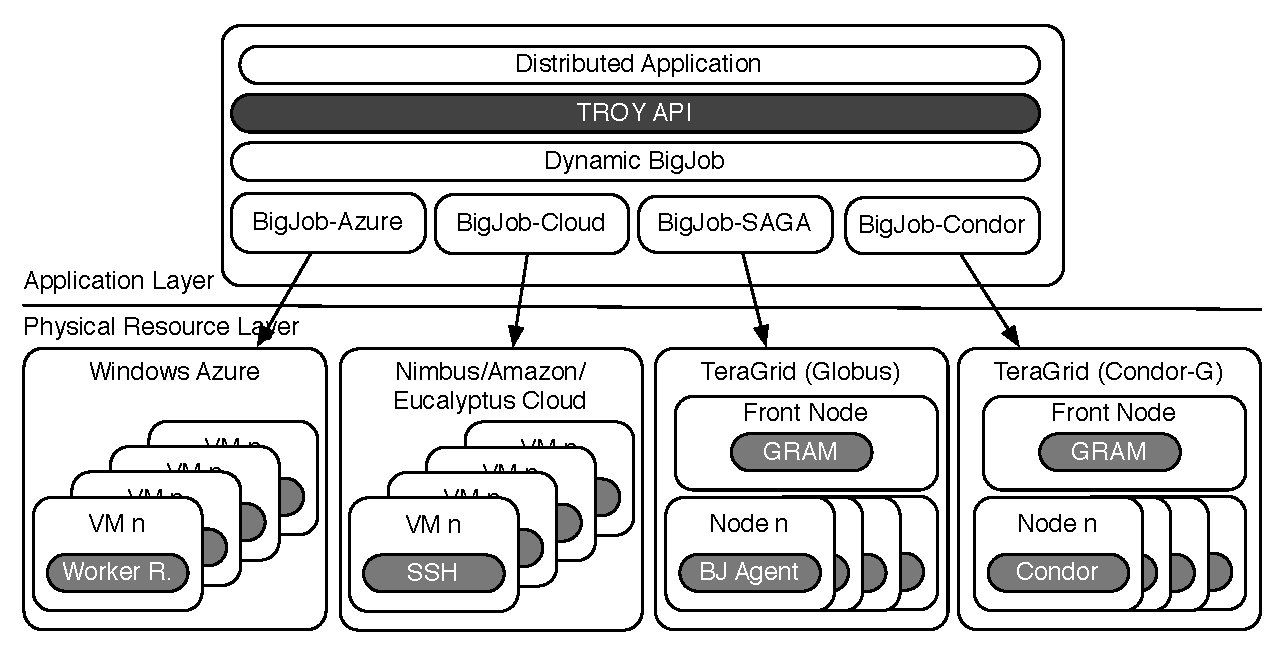
\includegraphics[width=0.7\textwidth]{figures/distributed_pilot_job.pdf}
%    \caption{BigJob API and Implementation}
%    \label{fig:figures_distributed_pilot_job}
%\end{figure}

BigJob is the SAGA-based Pilot-Job implementation of the TROY
framework. It supports a wide range of application types, and is
usable over a broad range of infrastructures, i.\,e.\ it is
general-purpose and extensible.  To aid the understanding of the
framework we define two kind of BigJobs, the atomic and the dynamic
BigJob:
\begin{itemize}
   \item  \textbf{Atomic BigJob:} An atomic BigJob is confined to a single 
   cluster resource and represented by a single master process (i.\,e.\ a 
   single BigJob Manager or DIANE RunMaster).
	\item \textbf{Dynamic BigJob:} A dynamic BigJob consists of several 
	pilot-jobs distributed across 1 or more resources. Dynamic BigJobs are 
	malleable, i.\,e.\ resources can added or be removed.
\end{itemize}

\jhanote{It is CRITICAL to explain why we need to expose the details
  of multiple atomic BigJobs to the end-user? Remember part of the
  whole idea of the exercise is, (i) theory: to provide a framework
  for understanding any differences, (ii) practise: make all these
  differences go away from the end user!}

The BigJob framework provides several types of atomic BigJob for
various resource types. The dynamic BigJob is discussed in
section~\ref{sec:dynamic_bigjob}.


Aspects that need to be addressed:
\begin{itemize}
    \item Big-Job Agent: capacity (physical size) is a property of an agent. 
	cardinality: how many sub-jobs can be managed by an agent?
	\item Sub-Job Agent: Agent assignment should be separated from resource 
	assignment. Agent has the freedom to assign tasks to sub-job in any way 
	it want. Agent can do local decisions.    
  \item Would it make sense to use the ``internal'' versus
    ``external'' coordination concept to distinguish sub-job
    versus big-job agent
\end{itemize}

\subsubsection{Dynamic BigJob}

\label{sec:dynamic_bigjob}
A traditional BigJob is always confined to a single resource. In many scenarios 
it is beneficial to utilize multiple resources, e.\,g.\ to accelerate the
time-to-completion or to provide resilience to resource failures and/or
unexpected delays. The Dynamic BigJob provides an abstraction for multiple
big-jobs. These big-jobs can be distributed across multiple resources and types
of infrastructures. Each big-job manages it's own resources. An extensible
scheduler is used for dispatching sub-jobs to the different big-jobs that are
managed by a dynamic big-job.


Dynamic BigJob provides the ability to dynamically add and remove resources to a 
big-job. The API consists of two parts, the resource management and the resource 
introspection part:
\begin{itemize}
    \item \texttt{add\_resource()}: New resources are added by starting a new
    big-job.There are various flavors of this method:
    \begin{itemize}
        \item \texttt{add\_resource(re\-sour\-ce\_dic\-tionary)}: Start another big-job on the resource defined in the \texttt{resource\_dictionary}.
        \item \texttt{add\_resource(affinity, number\_cores)}: Add another big-job to the specified affinity group.
    \end{itemize}
    \item \texttt{remove\_resource(bigjob)}: Removes the big-job from the
    resources.
\end{itemize}

Higher-level wrappers that encapsulate e.\,g.\ the specific resource
descriptions can be implement. Further, to implement this dynamic resource
capabilities it is necessary to provide different dynamic resource introspection
in the dynamic big-job layer:
\begin{itemize}
    \item \texttt{get\_resources()}: returns a list of managed big-job objects.
     Each big-job object can be queried for it's allocated resources (number 
     nodes, number cores).
\end{itemize}


% It uses SAGA BigJob approach to start multiple BigJobs agents 
% whether on a single resource or on multiple resources. And 
% these agents are responsible for pulling the tasks from advert 
% service and run the possible subjobs concurrently or in generations.

\jhanote{The rationale behind dynamic BJ is that for the same
  application scenario different BJ with different
  properties/characteristics may be required. Thus dynamic BJ maybe
  comprised of either homogeneous or heterogeneous atomic BJs}

In particular for data-intensive applications data locality is an important
concern. Different types of affinity, e.\,g.\ data-data or data-compute, exists.
Dynamic BigJob provides support for data-compute affinities. Each resource
(i.\,e.\ each big-job) can be assigned to a certain affinity. The affinity-aware
scheduler then ensures that sub-jobs that demand a certain affinity are only
executed on resources that fulfill this constraint.



\subsection{BigJob for Cloud Computing}

\jhanote{Once again -- why do differences in execution details between
  grids and clouds result in the need for different atomic BJs needs
  to be explained. Must emphasis that the API remains the same.}

At the execution level, clouds differ from Clusters/Grids in at least a couple
of different ways. In cloud environments, user-level jobs are not typically
exposed to a scheduling system; a user-level job consists of requesting the
instantiation of a virtual machine (VM). Virtual machines are either assigned to
the user or not (this is an important attribute that provides the illusion of
infinite resources). The assignment of job to a VM must be done by the user (or
a middleware layer as BigJob). In contrast, user-level jobs on grids and 
clusters are exposed to a scheduling system and are
assigned to execute at a later stage. Also a description of a grid job typically
contains an explicit description of the workload; in contrast for Clouds a user
level job usually contains the container (description of the resource
requested), but does not necessarily include the workload. In other words, the
physical resources are not provisioned to the workload but are provisioned to
the container.  Interestingly, at this level of formulation, pilot-jobs attempt 
to provide a similar model of resource provisioning as clouds natively offer. 

\subsubsection{BigJob and SAGA AWS Adaptor}

BigJob provides support for various cloud computing environment. The SAGA BigJob
implementation can be used in conjunction with the AWS adaptor for SAGA to run
on EC2-based cloud infrastructures, such as FutureGrid. However, there are some 
limitations mainly caused by the restrictions of SAGA/AWS adaptor for the SAGA 
Job package. The SAGA job service object e.\,g.\ does not provide a mean to 
specify a set of resources. Using the AWS adaptor it is only possible to utilize 
a single VM instance, which must be configured prior to the run in a 
configuration file. If multiple VMs are required, the dynamic BigJob 
implementation must be used. In this case however, it is still not possible to 
run MPI jobs across multiple VMs. 
\smnote {why is it not possible to run MPI jobs across Multiple VM's?} \alnote{MPI jobs are (unless you do something outside of BJ) constraint to run
on resources managed by a single BJ agent. The agent must generate a nodefile
from this list of resource it is managing. The agent is not aware of resources
managed by another BJ)}

\subsubsection{BigJob Cloud \& BigJob Azure}

To address this limitation, BigJob-Cloud~\cite{saga_bigjob_condor_cloud} was
developed. BigJob-Cloud provides an implementation of the BigJob API, which is
completely independent from the SAGA (and thus, the SAGA AWS adaptor). It
directly utilizes the Amazon tools to access cloud resources. It can manage
cluster of VM; for this purpose BigJob provides a rich interface for describing
cloud resources. For this purpose a Python dictionary is used (see
section~\ref{sec:api}). The VMs can be managed centrally by the BigJob manager:
All VMs have a public IP and there is no need to interface with a local resource
manager (SAGA BigJob e.\,g.\ evaluates the \texttt{\$PBS\_NODEFILE} to obtain a
list of resources). Thus, it is not necessary to deploy an agent on the VM - all
necessary metadata can be obtained from the AWS backend. Job are spawned via
SSH.

% \begin{itemize}
%   \item ManyJob is required to manage the set of VMs. The BigJob-Cloud can manage a set of VMs without the need of ManyJob.
%   \item Bigjob uses advert server for communication between BigJob-agent and BigJob whereas BigJob-Cloud does not use an advert server.
%   \item Bigjob-cloud does not require SAGA-AWS adaptors as opposed to requirement in original Bigjob. 
% \end{itemize} 


BigJob-Azure~\cite{10.1109/CloudCom.2010.85} utilizes a similar approach as
BigJob-Cloud. It utilizes the Azure REST interface to startup VM Worker Roles.
However, since Azure does not support SSH access it is necessary to utilize an
agent-based approach. For communication between the agent and the manager the
Azure Storage is used.

\msnote{If BigJob is the atomic unit, it should not differ per
  backend}\alnote{That's mainly a restriction of the job package which
  does not really map to AWS. There is no common way in the job
  package to specify the \# of resources that suppose to be
  used. Thus, this limitation}


\subsection{Pilot Data and Store}

\jhanote{We should purely by analogy go with BigData, no? Need a
  diagram that talks about TROY = BigJob + BigData + ``??''. Need to
  define ``??''}

\jhanote{note: DARE == Dynamic Application Runtime Environment: TROY +
  MapReduce + Other capabilities}

\jhanote{Ideally the background/underlying theory of Pilot Data/Store
  should be presented outside of TROY -- not sure this will be
  possible, or where, possibly in the \S II? Maybe as an explicit \S
  II-D, where we say, ``having defined a P-* model, we extend it to
  Dynamic Data..}

\label{sec:pilot-data}
\begin{figure}[t]
    \centering
        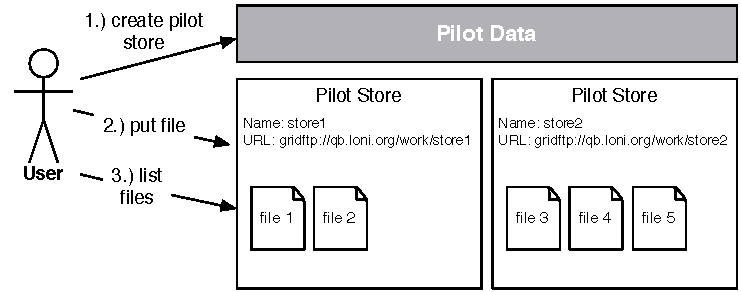
\includegraphics[width=0.45\textwidth]{figures/pilotstore.pdf}
    \caption{Pilot Data and Store Overview}
    \label{fig:figures_pilotstore}
\end{figure}

Pilot Data is a set of abstractions for expressing data localities and
affinities. Pilot Data can be used to create groups of file clustered
together using a quantifiable property, such as affinity ($\alpha$)
e.g., $\alpha = 1.0$ would imply that files are always stored
together. \jhanote{I've distinguished store and usage} The concept of
correlated access originates in
Filecules~\cite{Doraimani:2008:FGS:1383422.1383429}.

Pilot Data provides a set of basic operations on top of these file
groups, whilst Pilot Store is a container that represents a logical
group of physical files that share the same affinity.

Pilot Store Containers can be used to express data-data abstractions. 
Abstraction supports basic management tasks (create, delete, update,
move, list). 

\subsubsection{Overview}

The Pilot Data abstraction serves the following needs:
\begin{itemize}
	\item Reservation of physical disk space: acquisition of data storage (advanced reservation, place holder)
	\item Virtual destination: dynamically mapping of data to pilot stores.
	\item Runtime environment for $\alpha$ based data
	\item Automatic data partitioning and distribution
\end{itemize}


The pilot data abstraction provides two kinds of abstractions (see Figure~\ref{fig:figures_ps-instantiation}):
\begin{itemize}
    \item Pilot Data: Allows the logical grouping of files and the expression of data-data affinities. This collection of files can be associated with certain properties. One of this property is affinity.
    
    \item Pilot Store: Binds a pilot-data object to a actual physical resource. A pilot-store object can function as a placeholder object that reserves the space for a pilot-data object.
\end{itemize}


Figure~\ref{fig:figures_ps-instantiation} describes the differences between
pilot data object (abstract pilot stores) and pilot stores. A pilot data object
is a logical container and describes the properties of a group of files. A pilot
store is a placeholder reserving a certain amount of storage. By associating a
pilot data object to a pilot store the data is actually moved to the physically
location managed by the pilot store.

\begin{figure}[htbp]
    \centering
        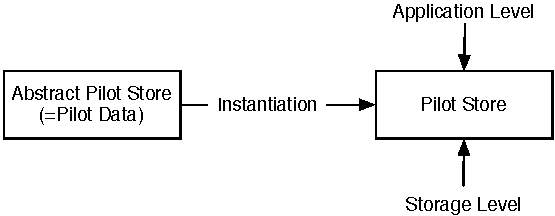
\includegraphics[width=0.45\textwidth]{figures/ps-instantiation.pdf}
    \caption{Level of Abstractions - Resource Binding}
    \label{fig:figures_ps-instantiation}
\end{figure}



	
\noindent	
Dynamic data:
\begin{itemize}
	\item Data to be generated (temporal)
	\item Data that is in place (spatial)
	\item Data that is changing (temporal)
	\item Data characteristics, properties
\end{itemize}	

\noindent
Analogies with Pilot-Job:
\begin{itemize}
	\item Assign pilot job to resource: $f^{1}(PJ_i) \rightarrow R_i$
	\item Assign task to pilot-job: $f^{2}(T_i) \rightarrow PJ_i$ 

	\item $g^{1} (D_i) \rightarrow PS_i$
	\item $g^{2} (PS_i) \rightarrow R_i$
\end{itemize}

\subsubsection{Pilot Data Architecture}

\jhanote{theory goes upfront; implementation and architecture stays
  here}

Data placement and locality is the key for a optimal performance of
data-intensive applications. The Pilot Data Manager is responsible for
optimizing the overall data distributions with respect to the
application requirements. The architecture is designed as a
\textbf{user-level overlay} on top of existing storage resources.

Figure~\ref{fig:figures_distributed_pilot_job} gives an overview of the
architecture. The system consists of two components: the pilot data manager and
the agents deployed on a specific physical storage resource. The manager is
responsible for 1) meta-data management, i.\,e.\ it keeps track of the pilot
stores that a pilot data object is associated with and 2) it schedules data
movements and data replications.

\jhanote{Need to explain/describe architecture of BigData? using the
  terminology of Section II and P*-Model}

\begin{figure}[htbp]
    \centering
        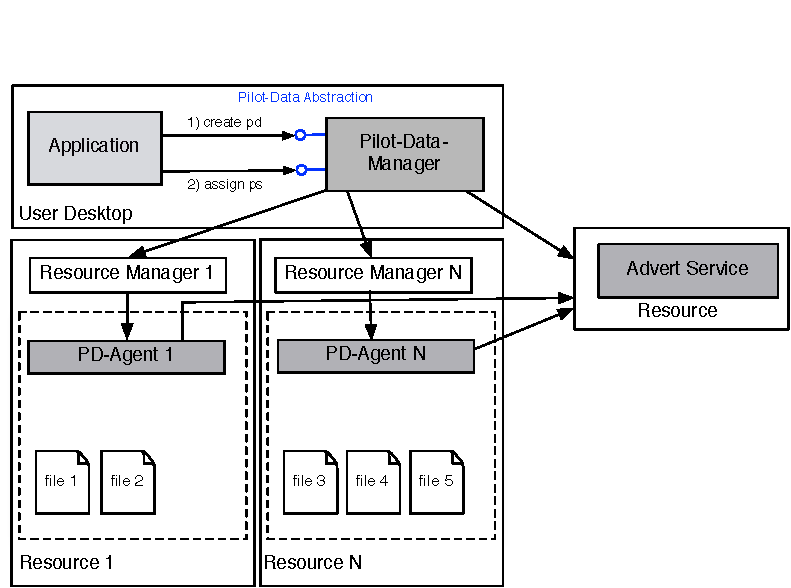
\includegraphics[width=0.4\textwidth]{figures/pilot-data-manager.pdf}
    \caption{Pilot Data Architecture}
    \label{fig:figures_distributed_pilot_job}
\end{figure}

Each pilot store is managed by an agent. The agent can be started manually or 
using the Pilot Data API. A possible implementation option would be the 
integration of the PD and BigJob agent, which is particularly useful for 
managing data-/compute-affinities.

A core part of the data manager is the data scheduler. The scheduler aims for a 
optimum of data and compute locality for an applications.
\begin{itemize}
	\item Move data to compute
	\item Move computer to data
	\item Streaming of data
	\item Data prefetching 
	\item Replication
\end{itemize}



\subsubsection{Data Movement}

The Pilot Data implementation is based on SAGA and thus, is infrastructure
independent. It supports all underlying SAGA adaptors (SSHFS, GridFTP) and
future adaptors such as Globus Online.

Work on optimizing file transfers: Kosar[2011]

Work on reliable file transfer: RFT, Globus Online


\subsubsection{Related Work}

\emph{iRods}


\emph{Stork}


\emph{BitDew}

Random Notes
\begin{itemize}
	\item Focus on Desktop Grid
	\item Java-based implementation (ie difficult to interface with Python-based PS/SAGA)
	\item highly distributed: stable and volatile nodes
	\item pull model, i.e. a node pulls for new data
\end{itemize}


Mapping to BitDew:
\begin{itemize}
	\item Pilot Store in its current implementation covers Bitdew Data Catalog and Repository
	\item For data management and placement the Active Data API and the Bitdew data scheduler could be used
	\item Transfer Management is done via SAGA File API	
\end{itemize}

How to evolve pilot data/store?
\begin{itemize}
	\item Active management of data (e.g. replication, automatic affinity management) requires an active component:
	\begin{itemize}
		\item Manager/Agent model as in BigJob?
		\item Who runs active components? Started as part of batch job or separate install/start?
	\end{itemize}
\end{itemize}

Questions:
\begin{itemize}
    \item How should
    we store data in order to effectively cope with non-uniform demand for
    data? 
    \item How many copies of popular data objects do we need? 
    \item Where should we store them for effective load balancing?
\end{itemize}

\subsection{TODO/Future Work}
The current framework provides building blocks for expressing data localities and operation on file groups (similar to filecules).

Limitations:
\begin{itemize}
    \item No active agent that monitors state of files
    \item No placement policy support or autonomic behavior
    \item Infrastructures generally expose insufficient locality/topology information
    \item Compute – Data Affinity: Dynamic BigJob with affinity only provides a very coarse-grained affinity
    \item No policy for what’s happening if data is not available in right location:
    \begin{itemize}
        \item Run anyways – affinity is just an hint
    \end{itemize}
    \item When to move pilot stores? Move or copy?
    \item Move data to compute or visa versa?
    \item Data Replication: Identification of the same file: logical filename -> physical files. Manage replication process (consistency!)
\end{itemize}



%%%%%%%%%%%%%%%%%%%%%%%%%%%%%%%%%%%%%%%%%%%%%%%%%%%%%%%%%%%%%%%%%%%%%%

\section{Understanding Other Pilot-Jobs \jhanote{MS - to focus on
    DIANE}}


\jhanote{Depending upon where the TROY API is discussed we can have
  two ways forward. If TROY API is discussed in \S 3, then we go for
  Mode I, where Mode I: The aim of this section is to show: (i) that
  our P* Model can be used to explain/understand DIANE, (ii) Show that
  the TROY API can be used to marshall Diane stand-alone, (iii) Using
  TROY API, both BigJob and Diane can be used standalone}

\jhanote{If TROY API is discussed in \S 5, then we go for Mode-II,
  where Mode II: The aim of \S 4 is to show: (i) that our P* Model can
  be used to explain/understand DIANE.  Then in \S 5, after having
  discussed TROY API we, (ii) Show that the TROY API can be used to
  marshall Diane stand-alone, (iii) Using TROY API, both BigJob and
  Diane can be used stand alone}


\subsection{Diane}

DIANE~\cite{Moscicki:908910} is a task coordination framework which implements 
the Master/Worker pattern. 

\subsubsection{Mapping of BigJob / Diane terms}

\begin{table*}[t]
\centering
\begin{tabular}{|p{3.5cm}|p{5.9cm}|p{5.7cm}|}
\hline
\textbf{Term} &\textbf{Atomic BigJob/Dynamic BigJob} &\textbf{Diane}  \\
\hline
Central Coordinator &BigJob/ManyJob Manager & RunMaster \\ 
\hline
Resource Agent / Pilot &BigJob Agent  & Worker Agent \\
\hline
Number Agents \jhanote{Whats an ``Agent''?}  &1 BJ Agent/n BJ Agents & 1 Worker Agent per core \\
\hline
Capacity of Agent &n cores & 1 core\\
\hline
Scheduleable Unit&Sub-Job &  Task \\
\hline
Communication &SAGA-Advert & CORBA\\
\hline
Support for task execution by generations  &yes &yes\\  
\hline
Task-resource Binding &Late (At sub-job submission or later for dynamic BJ) &Late\\
\hline
MPI/Multinode Applications &yes &no (yes with custom implementation of ApplicationWorker)\\
\hline
Advanced Scheduling &no/ManyJob Scheduler &yes (ITaskScheduler)\\
\hline
Dynamic Resources &no/yes &yes (AgentFactories)\\
\hline
Agent Submission &API &Ganga Submission Script\\
\hline
Application Interfaces &Big-Job/Sub-job Management &Big-Job/Sub-job 
Management\linebreak[4] Master/Worker API (\texttt{ITaskScheduler}, 
\texttt{IApplicationManager}, \texttt{IApplicationWorker}) \\
\hline
Fault Tolerance &Error Propagation &Configurable Re-Tries\\
\hline
\end{tabular}
\caption{BigJob / DIANE Terms and Features}
\end{table*}

\msnote{Whats VO in this context?}\alnote{Suppose to describes the capability to dynamically add/remove resource from/to a BigJob}


\alnote{Update: atomic pilot, multiple pilot model}


\subsection{DIRAC}

\jhanote{Dirac is not critical, and can be clubbed together with other
  PJ implementations described below}

DIRAC~\cite{1742-6596-219-6-062049} is another pilot-job framework used by the 
LHCb community.

\subsection{Other Pilot-Jobs}

\begin{itemize}
    \item MyCluster
    \item Swift
    \item Falkon
    \item Nimrod/G
    \item Dirac
    \item Topos
    \item Panda    
\end{itemize}

\jhanote{Can we add some structure to these *other* PJ.. this will be
  ambitious and time-consuming, but if we can, that'll be (i) a great
  service to the community, (ii) a strong intellectual addition to the
  paper by virtue of validation of the P*-model}

\jhanote{Saw the table after I wrote above jhanote. I should have
  known Andre L would have already done this! Great job! I agree --
  doing it for 4 PJs should be good enough}

\begin{table*}[t]
\centering
\begin{tabular}{|l|p{2.5cm}|p{2.5cm}|p{2.5cm}|p{2.5cm}|}
	\hline
	&\textbf{SAGA BigJob} &\textbf{DIANE} &\textbf{Condor Glide-In} &   
	\textbf{DIRAC} \\ \hline
External Coordination &Local API for UW execution management & &Master/Worker &\\ \hline

Internal Coordination &Master/Worker (push) &Master/Worker (pull/push) &Master/Worker &Master/Worker\\ \hline

External Communication &local &Central Manager exposes local \& remote CORBA service & &\\ \hline
	
Internal Communication &Advert Service &CORBA & & \\ \hline

UW Binding \& Scheduling &&&&\\ \hline

Security &Middleware dependent (GSI, Advert DB Login) &GSI &- &GSI/Glexec\\ \hline

Resource Types &HTC/HPC (via SAGA adaptors) &HTC &HTC &HTC \\ \hline

Fault Tolerance  &&&&\\ \hline
	
\end{tabular}
\caption{Pilot-Job Comparison}
\end{table*}

\section{Implementations and Experiments \jhanote{AL/MS, SM}}


\section{Conclusion and Future Work}



\bibliographystyle{plain}
\bibliography{pilotjob,saga.bib}
\end{document}
